%!TEX root = ../main.tex
\setcounter{chapter}{3}
\chapter{Navigation Function}
\section{code}
	\lstinputlisting[language=Matlab, firstline=7]{../../Matlab/solved/scripts/solvedCase4NavigationFunction.m}
	\newpage
	\lstinputlisting[language=Matlab, firstline=2]{../../Matlab/solved/functions/solvedNavigationFunction.m}
	\lstinputlisting[language=Matlab, firstline=2]{../../Matlab/solved/functions/solvedNavigationFunctionGradient.m}

	\begin{landscape}
\section{simulink}
	\begin{figure}[!h]
		\centering
		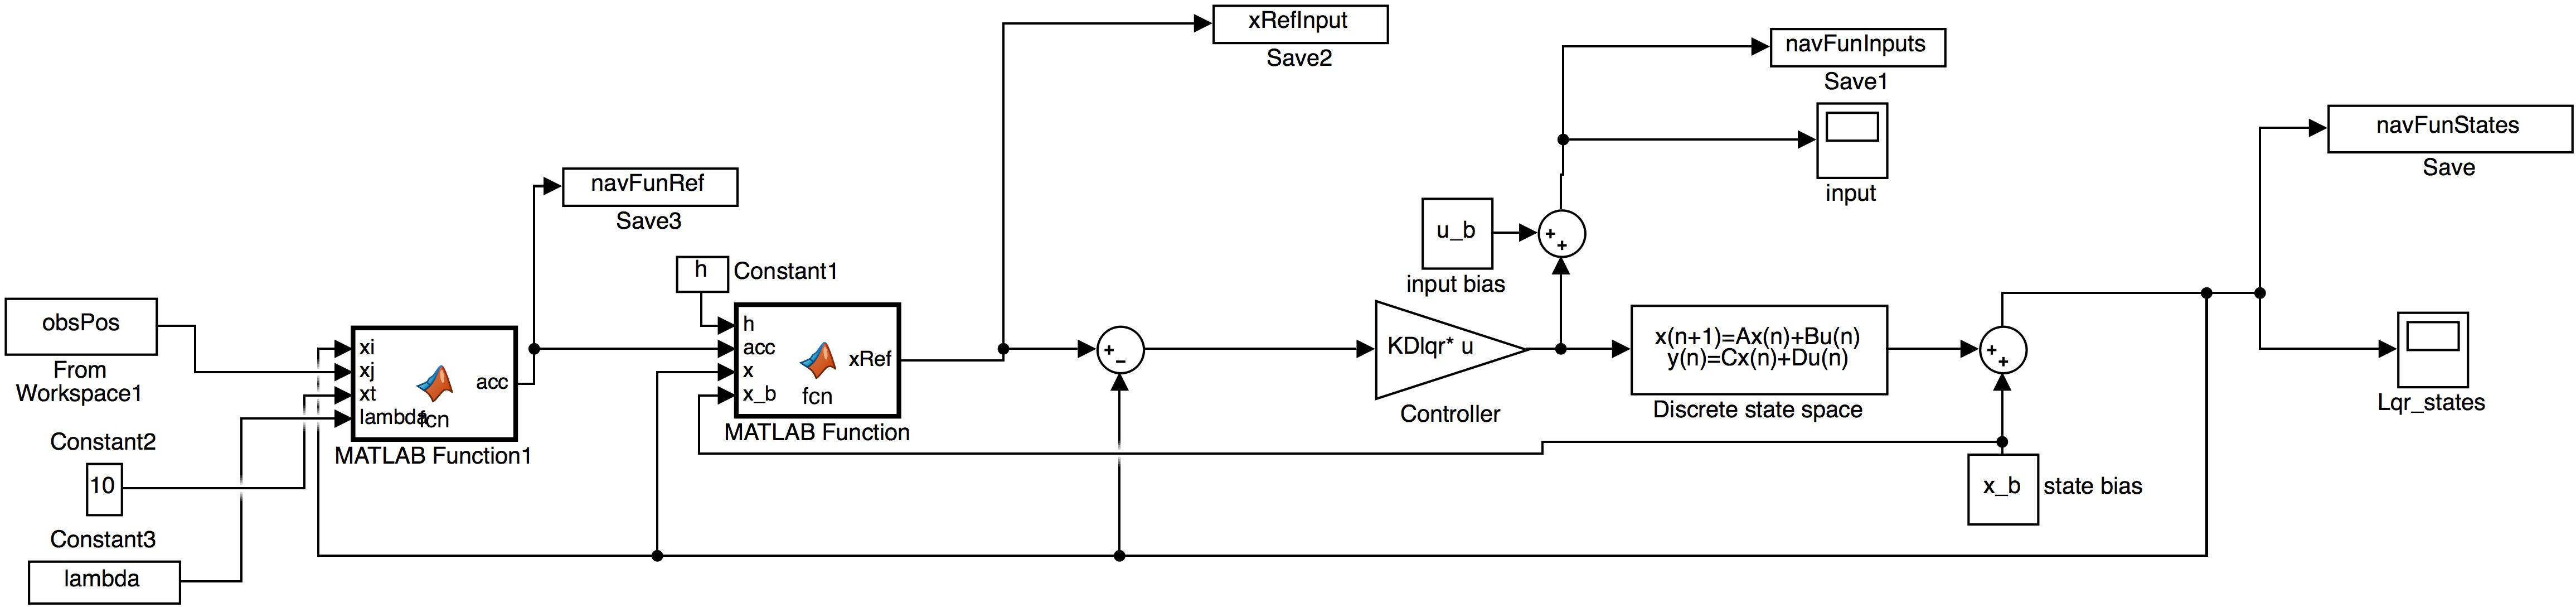
\includegraphics[width = \linewidth]{./Imag/solvedNavFunction}
		\caption{Simulink blocks to use : open loop longitudinal control}
		\label {fig:NavFunSimulink}
	\end{figure}
	\end{landscape}
